\documentclass[aspectratio=169,11pt]{beamer}

\usepackage[T1]{fontenc}
\usepackage[utf8]{inputenc}
\IfFileExists{newpxtext.sty}{
  \usepackage{newpxtext}
  \usepackage{newpxmath}
}{
  \usepackage{mathpazo}
}
\usefonttheme{serif}
\usepackage{amsmath}
\usepackage{booktabs}
\usepackage{graphicx}
\usepackage{microtype}
\usepackage[framemethod=default]{mdframed}
\usepackage{tikz}
\usetikzlibrary{arrows.meta,positioning}

% Paper-outline palette.
\definecolor{boxfill}{HTML}{EAF2FA}
\definecolor{boxrule}{HTML}{2C6EAB}
\definecolor{graytext}{HTML}{767676}
\definecolor{rulegray}{HTML}{BFBFBF}
\definecolor{trpbgreen}{HTML}{3F7A4F}
\definecolor{nucorange}{HTML}{D95F02}
\definecolor{textgray}{HTML}{4E535B}

\setbeamercolor{normal text}{fg=textgray,bg=white}
\setbeamercolor{structure}{fg=boxrule}
\setbeamercolor{frametitle}{fg=textgray,bg=white}
\setbeamercolor{block title}{fg=white,bg=boxrule}
\setbeamercolor{block body}{fg=textgray,bg=boxfill}
\setbeamercolor{alerted text}{fg=boxrule}
\setbeamercolor{upper separation line foot}{bg=rulegray}
\setbeamerfont{frametitle}{size=\Large,series=\bfseries}
\setbeamerfont{title}{size=\LARGE,series=\bfseries}
\setbeamerfont{subtitle}{size=\large}
\setbeamerfont{footline}{size=\scriptsize}
\setbeamertemplate{navigation symbols}{}
\setbeamertemplate{itemize item}{\color{boxrule}\raise0.15ex\hbox{\scriptsize$\blacktriangleright$}}
\setbeamertemplate{itemize subitem}{\color{boxrule}\raise0.15ex\hbox{\tiny$\bullet$}}
\setbeamertemplate{frametitle}{
  \vspace{0.14cm}
  \usebeamerfont{frametitle}\insertframetitle\par
  \vspace{0.04cm}
  {\color{rulegray}\hrule height0.45pt}
}
\setbeamertemplate{footline}{
  \leavevmode%
  \begin{beamercolorbox}[colsep=0.18pt]{upper separation line foot}\end{beamercolorbox}%
  \par\nointerlineskip
  \begin{beamercolorbox}[wd=\paperwidth,ht=0.33cm,dp=0.12cm,leftskip=0.5cm,rightskip=0.5cm]{author in head/foot}
    \color{graytext}\usebeamerfont{footline}%
    Deep mutational scanning and ranking resolution\hfill\insertframenumber
  \end{beamercolorbox}%
}

\newmdenv[
  backgroundcolor=boxfill,
  linecolor=boxrule,
  linewidth=2.4pt,
  topline=false,
  bottomline=false,
  rightline=false,
  leftline=true,
  innerleftmargin=8pt,
  innerrightmargin=8pt,
  innertopmargin=3pt,
  innerbottommargin=3pt,
  skipabove=2pt,
  skipbelow=2pt,
  roundcorner=0pt
]{callout}

\newcommand{\key}[1]{\textcolor{boxrule}{\bfseries #1}}
\newcommand{\muted}[1]{\textcolor{graytext}{#1}}
\newcommand{\tightitems}{\setlength{\itemsep}{0.35em}\setlength{\parskip}{0pt}}
\newcommand{\source}[1]{\vspace{0.2em}{\tiny\color{graytext}#1}}
\graphicspath{{assets/}{../../output/hmc/figures/}{../../output/mle_predictive/figures/}}

\title[Ranking resolution in DMS]{How much ordering information does a deep mutational scan contain?}
\subtitle{Quantifying ranking resolution in protein fitness landscapes}
\author{Renato Berlinghieri}
\date{Collaborator meeting \textbar{} 31 August 2026}

\begin{document}

% 0:30
\begin{frame}[plain]
  \begin{tikzpicture}[remember picture,overlay]
    \fill[boxfill] (current page.south west) rectangle ([yshift=1.15cm]current page.south east);
    \fill[boxrule] (current page.north west) rectangle ([xshift=0.17cm]current page.south west);
  \end{tikzpicture}
  \vspace{0.65cm}
  {\fontsize{20.74pt}{23pt}\selectfont\bfseries\color{textgray}\inserttitle\par}
  \vspace{0.28cm}
  {\usebeamerfont{subtitle}\color{boxrule}\insertsubtitle\par}
  \vspace{0.5cm}
  \color{rulegray}\rule{0.72\linewidth}{0.6pt}
  \vspace{0.5cm}

  {\large\insertauthor\par}
  \vspace{0.12cm}
  {\color{graytext}\insertdate\par}

  \vfill
  {\small\color{graytext}
    Main question: which parts of a DMS ordering are actually supported by the observed counts?
  }
\end{frame}

% 1:30
\begin{frame}{A DMS measures counts; the ranking is constructed}
  \centering
  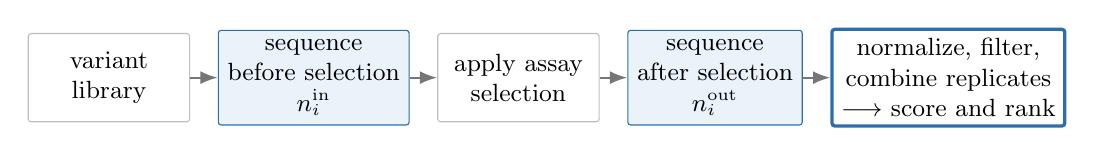
\begin{tikzpicture}[
    node distance=0.35cm,
    stagebox/.style={
      draw=rulegray,
      fill=white,
      rounded corners=1pt,
      minimum width=2.05cm,
      minimum height=1.12cm,
      align=center,
      font=\small
    },
    measured/.style={stagebox,fill=boxfill,draw=boxrule},
    arrow/.style={-{Latex[length=2.2mm]},thick,draw=graytext}
  ]
    \node[stagebox] (library) {variant\\library};
    \node[measured,right=of library] (input) {sequence\\before selection\\$n_i^{\mathrm{in}}$};
    \node[stagebox,right=of input] (selection) {apply assay\\selection};
    \node[measured,right=of selection] (output) {sequence\\after selection\\$n_i^{\mathrm{out}}$};
    \node[stagebox,right=of output,draw=boxrule,line width=1.2pt] (rank) {normalize, filter,\\combine replicates\\$\longrightarrow$ score and rank};
    \draw[arrow] (library) -- (input);
    \draw[arrow] (input) -- (selection);
    \draw[arrow] (selection) -- (output);
    \draw[arrow] (output) -- (rank);
  \end{tikzpicture}

  \vspace{0.35cm}
  \begin{columns}[T,onlytextwidth]
    \column{0.47\textwidth}
      \key{Direct observations}
      \begin{itemize}\tightitems
        \item counts at finite sequencing depth
        \item replicate, timepoint, or gate structure
      \end{itemize}
    \column{0.47\textwidth}
      \key{Analysis choices}
      \begin{itemize}\tightitems
        \item score definition and normalization
        \item filtering and replicate aggregation
      \end{itemize}
  \end{columns}

  \begin{callout}
    A published score table is an \textbf{analysis output}, not a direct measurement of an assay-independent fitness.
  \end{callout}
\end{frame}

% 1:30
\begin{frame}{The same point estimate can have very different support}
  \begin{columns}[T,onlytextwidth]
    \column{0.43\textwidth}
      \centering
      \vspace{0.2cm}
      \begin{tabular}{lrrc}
        \toprule
        & input & output & ratio \\
        \midrule
        sparse & 1 & 10 & 10 \\
        deep & 1,000 & 10,000 & 10 \\
        \bottomrule
      \end{tabular}

      \vspace{0.45cm}
      {\small A one-read change alters the first ratio substantially, but hardly moves the second.}

    \column{0.52\textwidth}
      \key{Two distinct sources of ambiguity}
      \begin{enumerate}
        \item \textbf{Definition dependence:} reasonable score constructions can produce different orderings.
        \item \textbf{Finite resolution:} after fixing one analysis, finite counts leave uncertainty about the induced ordering.
      \end{enumerate}
  \end{columns}

  \vspace{0.15cm}
  \begin{callout}
    \centering
    \large\itshape How much of the ordering induced by a DMS landscape is supported by the observed counts?
  \end{callout}
\end{frame}

% 1:30
\begin{frame}{Why ranking resolution matters}
  \small
  \begin{columns}[T,onlytextwidth]
    \column{0.47\textwidth}
      \begin{block}{Protein engineering}
        \begin{itemize}\tightitems
          \item Which variants should be validated?
          \item Which mutations should be combined?
          \item How many candidates are genuinely distinguishable near the cutoff?
        \end{itemize}
      \end{block}

    \column{0.47\textwidth}
      \begin{block}{Machine-learning evaluation}
        \begin{itemize}\tightitems
          \item Spearman and top-$K$ metrics depend on label ordering.
          \item A small model difference may be real but unresolved by the experiment.
          \item Benchmark labels should not imply more precision than the counts contain.
        \end{itemize}
      \end{block}
  \end{columns}

  \begin{callout}
    The useful output is often a \textbf{candidate set with inclusion probabilities} and a resolution scale, not an exact ranking.
  \end{callout}
\end{frame}

% 2:00
\begin{frame}{What we quantify, and why the construction is useful}
  \small
  \begin{columns}[T,onlytextwidth]
    \column{0.47\textwidth}
      \begin{block}{HMC posterior}
        \begin{itemize}\tightitems\footnotesize
          \item Fit a generative count model.
          \item Sample latent assay-score landscapes.
          \item Include fitted-score parameter uncertainty.
        \end{itemize}
      \end{block}
    \column{0.47\textwidth}
      \begin{block}{MLE predictive}
        \begin{itemize}\tightitems\footnotesize
          \item Fix parameters at the MLE.
          \item Sample repeated count experiments.
          \item Recompute the source count-derived score.
        \end{itemize}
      \end{block}
  \end{columns}

  \vspace{0.18cm}
  \centering
  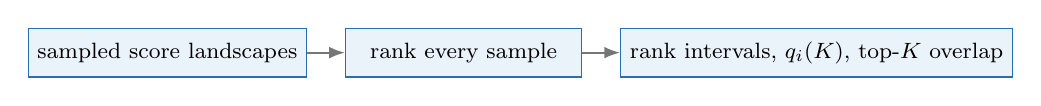
\begin{tikzpicture}[
    node distance=0.48cm,
    common/.style={draw=boxrule,fill=boxfill,minimum height=0.62cm,align=center,font=\footnotesize},
    arrow/.style={-{Latex[length=2mm]},thick,draw=graytext}
  ]
    \node[common,minimum width=3.1cm] (scores) {sampled score landscapes};
    \node[common,right=of scores,minimum width=3.0cm] (ranks) {rank every sample};
    \node[common,right=of ranks,minimum width=4.3cm] (metrics) {rank intervals, $q_i(K)$, top-$K$ overlap};
    \draw[arrow] (scores) -- (ranks);
    \draw[arrow] (ranks) -- (metrics);
  \end{tikzpicture}

  \begin{callout}
    \footnotesize The procedures answer \textbf{different uncertainty questions}; their numerical intervals are not interchangeable.
  \end{callout}
\end{frame}

% 2:00
\begin{frame}{Experimental systems and current analysis scope}
  \centering
  \scriptsize
  \begin{tabular}{p{1.15cm}p{3.0cm}cccc}
    \toprule
    system & assay/readout & landscapes & fitted variants & HMC runs & MLE-pred. runs \\
    \midrule
    \textcolor{boxrule}{\bfseries PDZ} & peptide binding & 5 & 10.7k--151.6k & 14 & 19 \\
    \textcolor{trpbgreen}{\bfseries TrpB} & enzyme activity coupled to growth & 10 & 9.0k--194.4k & 28\,$^{a}$ & 34 \\
    \textcolor{nucorange}{\bfseries NucB} & fluorescence-sorted nuclease activity & 4 & 10.8k--18.8k & 7 & 7 \\
    \midrule
    \textbf{total} & & \textbf{19} & & \textbf{49} & \textbf{60} \\
    \bottomrule
  \end{tabular}

  \source{$^{a}$HMC covers nine TrpB landscapes; four-site is MLE-only. Cross-procedure figures use the 18 shared landscapes. Sources: Zarin et al.; Johnston et al.; Thomas et al.}

  \vspace{0.12cm}
  \begin{columns}[T,onlytextwidth]
    \column{0.31\textwidth}
      \key{Alignment}
      \footnotesize Raw counts, fitted axes, and candidate/control roles are checked.
    \column{0.31\textwidth}
      \key{Score checks}
      \footnotesize TrpB and NucB source scores are reproduced exactly.
    \column{0.31\textwidth}
      \key{Predictive checks}
      \footnotesize All 60 MLE artifacts pass shape and fixed-total checks.
  \end{columns}

  \begin{callout}
    \footnotesize PDZ MLE results use a provisional DiMSum-style proxy.
  \end{callout}
\end{frame}

% 1:30
\begin{frame}{The published ordering is not always recovered}
  \centering
  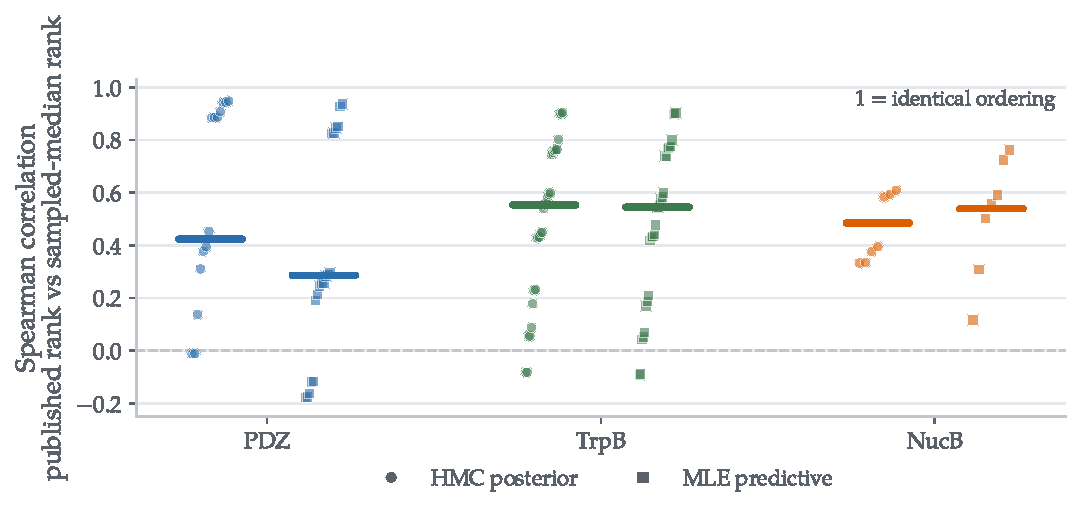
\includegraphics[height=4.8cm,keepaspectratio]{reported_concordance.pdf}
  \begin{callout}
    \footnotesize Points are analysis runs; bars are landscape-weighted medians. Agreement ranges from near zero or slightly negative to above 0.9.
  \end{callout}
\end{frame}

% 1:30
\begin{frame}{A precise top ten is not ten precisely resolved positions}
  \begin{columns}[T,onlytextwidth]
    \column{0.73\textwidth}
      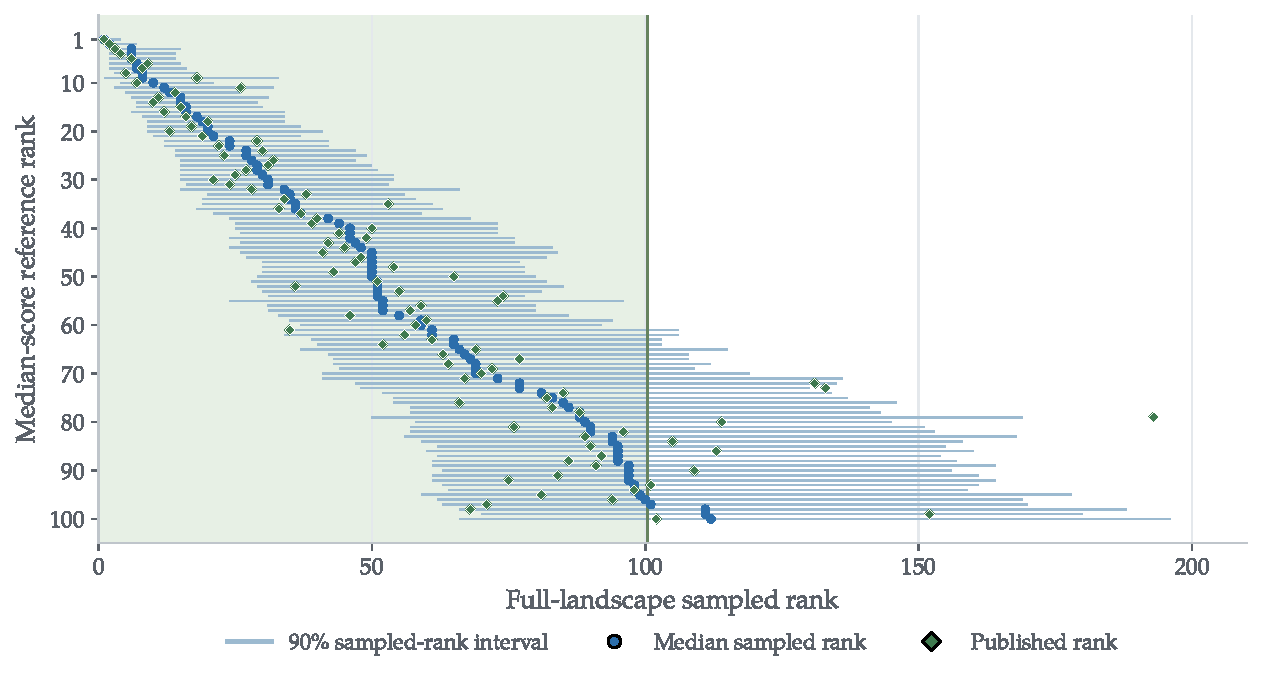
\includegraphics[height=3.9cm,width=\linewidth,keepaspectratio]{rank_example_pdz.pdf}
    \column{0.24\textwidth}
      \vspace{0.25cm}
      \footnotesize
      \key{PDZ cis example}
      \begin{itemize}\tightitems
        \item Rows are ordered by median fitted score.
        \item Lines show 90\% sampled-rank intervals.
        \item Several top-ten intervals overlap and extend beyond rank 10.
      \end{itemize}

  \end{columns}

  \begin{callout}
    \footnotesize The experiment can identify a promising region without resolving the exact order inside it.
  \end{callout}
\end{frame}

% 2:00
\begin{frame}{Top-100 rank resolution varies by system and analysis}
  \centering
  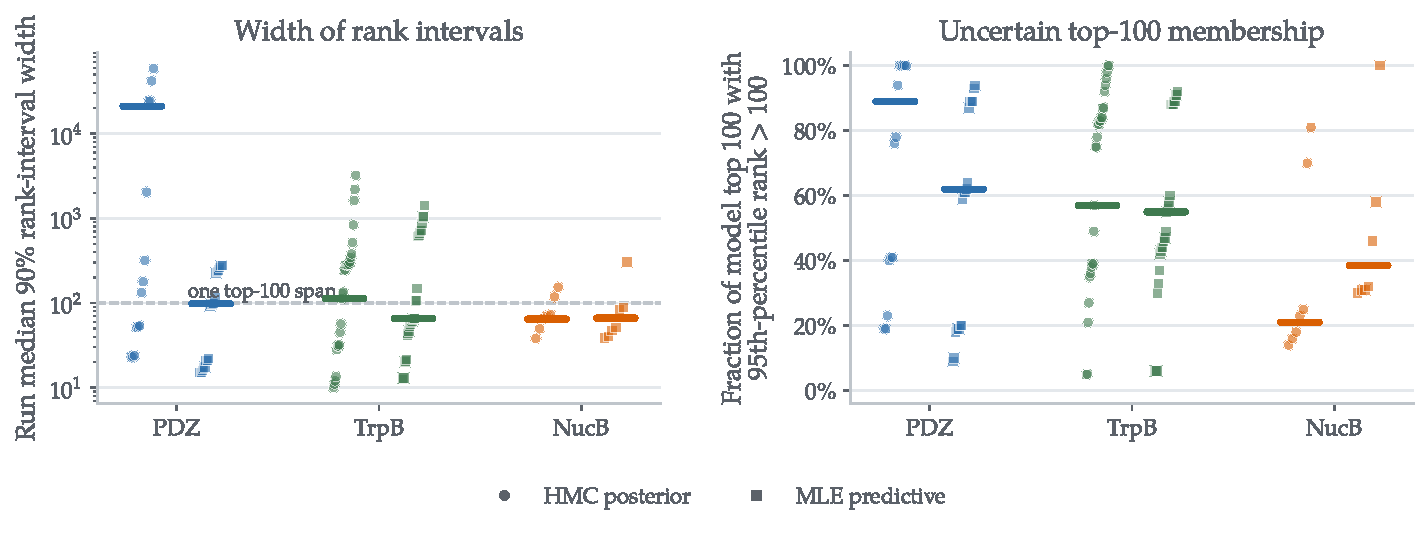
\includegraphics[height=4.8cm,keepaspectratio]{rank_resolution.pdf}
  \begin{callout}
    \footnotesize Landscape-weighted median top-100 exit fractions: HMC \textbf{89\% PDZ, 57\% TrpB, 21\% NucB}; MLE predictive \textbf{62\%, 55\%, 39\%}.
  \end{callout}
\end{frame}

% 2:00
\begin{frame}{Decision stability depends on both system and set size}
  \centering
  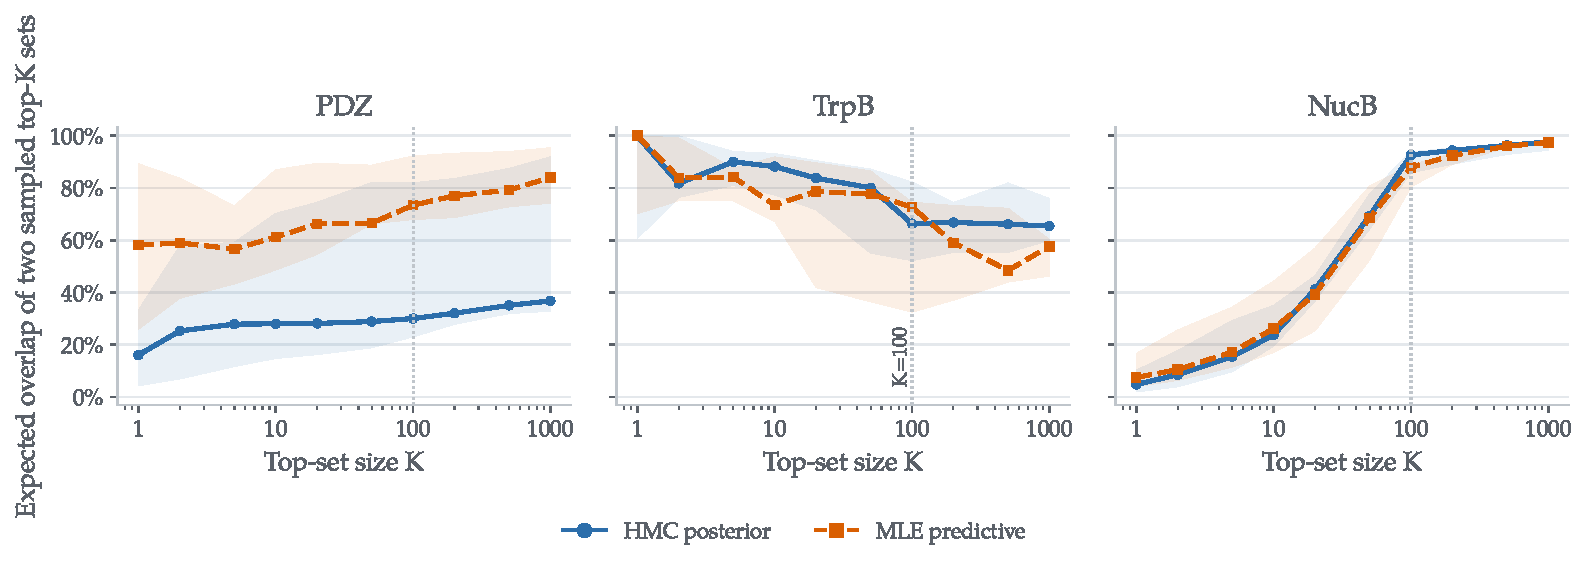
\includegraphics[height=4.25cm,keepaspectratio]{top_k_stability.pdf}
  \begin{columns}[T,onlytextwidth]
    \column{0.48\textwidth}
      \footnotesize\key{Metric:} expected fraction shared by two sampled top-$K$ sets.
    \column{0.48\textwidth}
      \footnotesize\key{Reading:} $K$ is part of the scientific decision, not a plotting choice.
  \end{columns}
  \begin{callout}
    \small Resolution can change sharply with $K$ and differs across uncertainty procedures.
  \end{callout}
\end{frame}

% 2:00
\begin{frame}{What is associated with ranking resolution?}
  \centering
  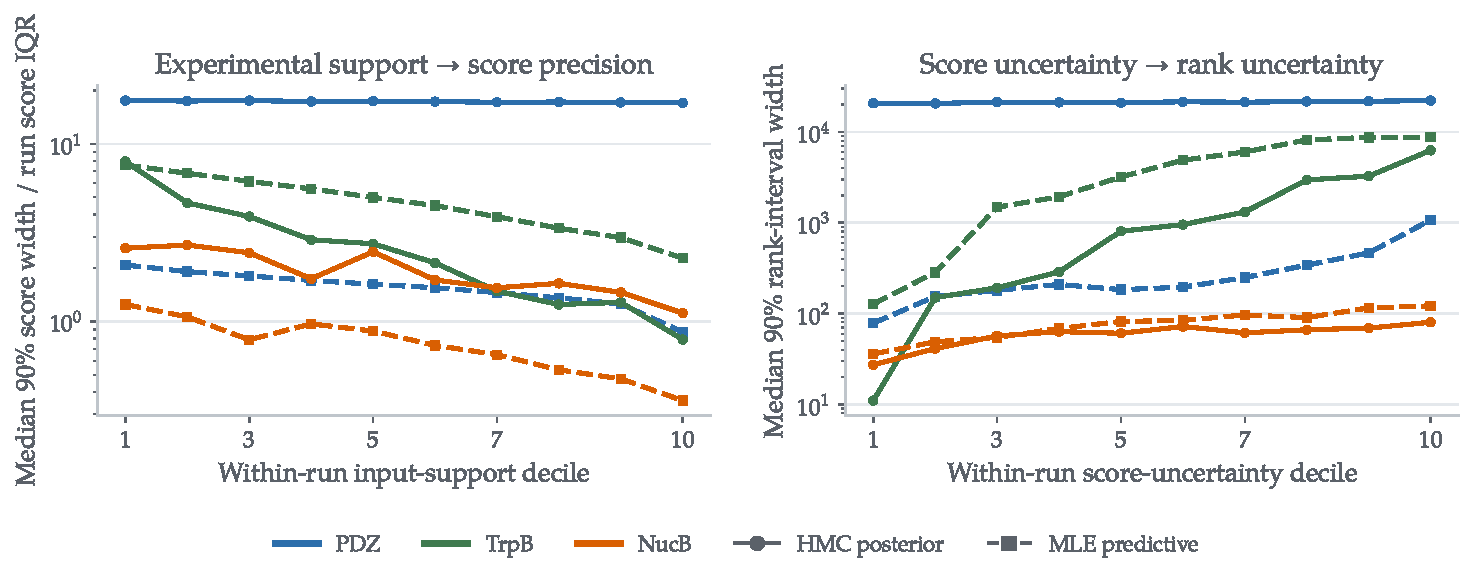
\includegraphics[height=4.25cm,keepaspectratio]{mechanism_chain.pdf}
  \begin{columns}[T,onlytextwidth]
    \column{0.48\textwidth}
      \footnotesize Higher input support is generally associated with narrower score intervals.
    \column{0.48\textwidth}
      \footnotesize Wider score intervals and local crowding are associated with wider rank intervals.
  \end{columns}
  \begin{callout}
    \small Descriptive associations only; they do not estimate the causal effect of adding reads.
  \end{callout}
\end{frame}

% 1:30
\begin{frame}{Similar instability can arise from different local patterns}
  \centering
  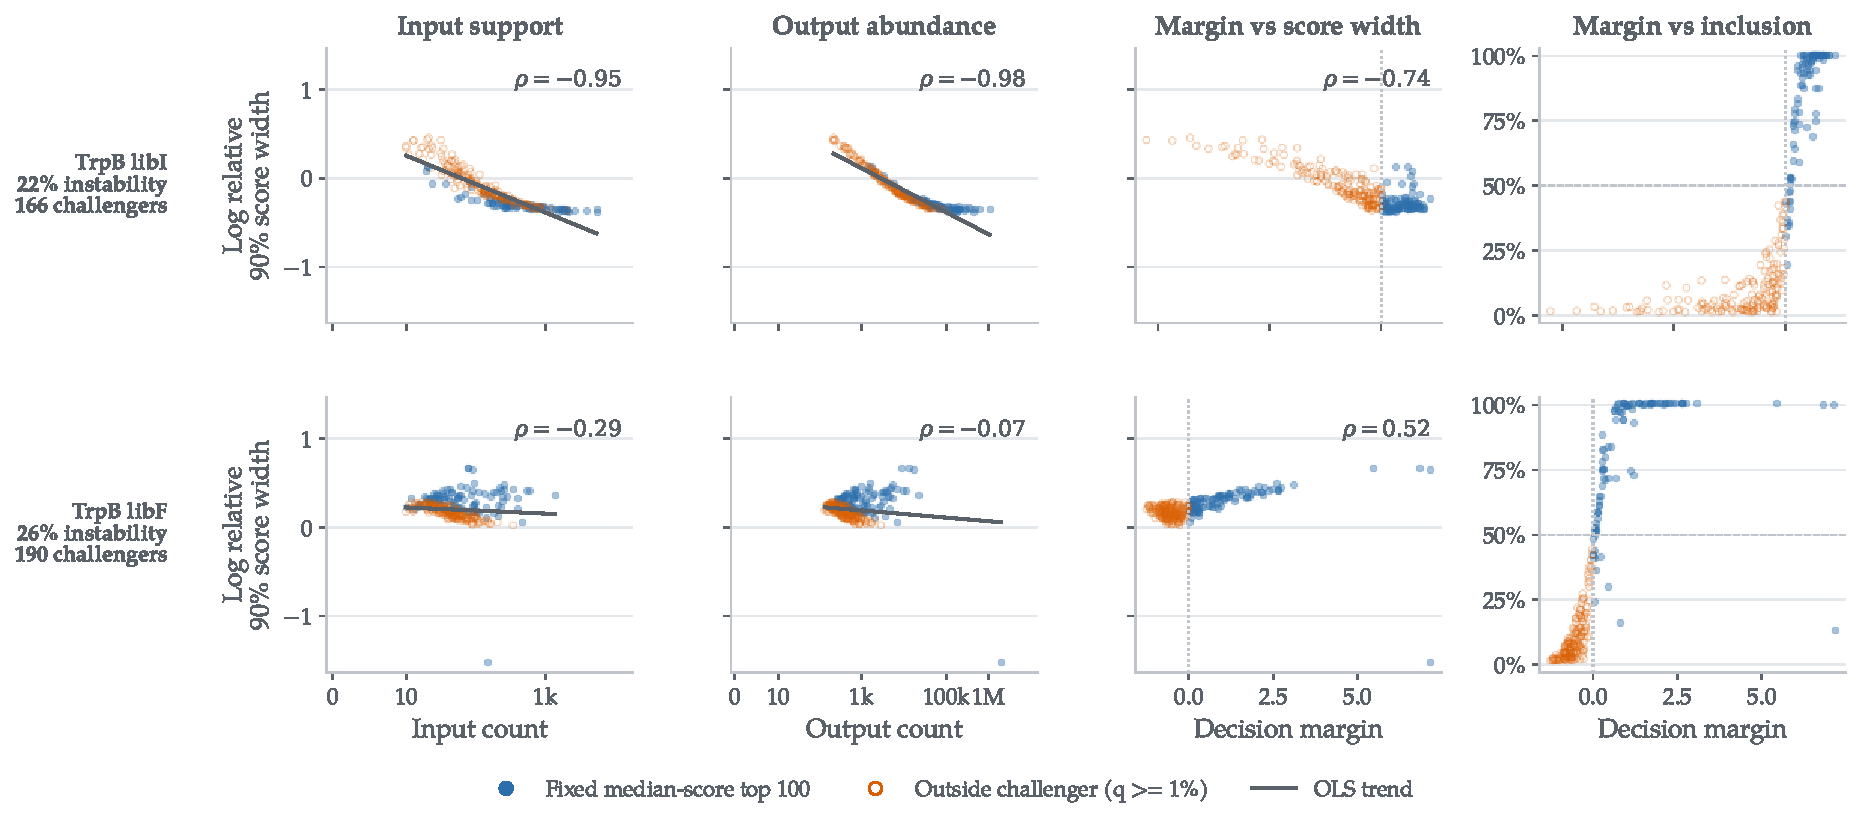
\includegraphics[height=4.55cm,keepaspectratio]{figure10_contrast.pdf}
  \begin{callout}
    \scriptsize Same protein, model, and uncertainty procedure; similar top-100 instability. LibI shows strong support--precision coupling and $\rho_{\mathrm{margin,width}}=-0.74$; libF shows weak count coupling and $\rho_{\mathrm{margin,width}}=+0.52$.
  \end{callout}
  \source{Deliberately selected Figure 10 contrast. Primary cohort = fixed top 100 plus outside candidates with $q_i(100)\geq0.01$. Decision-margin ranges are analysis-specific; exact zero widths use a plot-only floor.}
\end{frame}

% 1:00
\begin{frame}{What we can conclude, and what remains conditional}
  \footnotesize
  \begin{columns}[T,onlytextwidth]
    \column{0.47\textwidth}
      \begin{block}{Supported by the current analyses}
        \begin{itemize}\tightitems
          \item DMS orderings have finite, heterogeneous resolution.
          \item Reported and fitted central orderings can differ.
          \item Top-$K$ uncertainty can be expressed directly as decision probabilities.
          \item Count support and score geometry help explain where resolution is lost.
        \end{itemize}
      \end{block}
    \column{0.47\textwidth}
      \begin{block}{Not implied by the current analyses}
        \begin{itemize}\tightitems
          \item a universal, assay-independent true fitness
          \item MLE-predictive intervals as MLE confidence intervals
          \item a causal estimate of how much more sequencing would help
          \item that a published ranking is simply ``wrong''
        \end{itemize}
      \end{block}
  \end{columns}

  \begin{callout}
    \small \textbf{Recommendation:} report rank intervals, top-$K$ inclusion probabilities, and the assay/analysis definition with point scores.
  \end{callout}

  \centering
  \scriptsize\color{graytext}Discussion: which decision should define $K$, and how should label resolution enter benchmark comparisons?
\end{frame}

\begin{frame}{Backup: the three decision-level estimands}
  For sampled top-$K$ set $T_K^{(s)}$, fixed median-score set $T_K^\star$, and published set $T_K^{\mathrm{rep}}$:
  \begin{align*}
    C_K
      &= E_{s\ne s'}\left[\frac{|T_K^{(s)}\cap T_K^{(s')}|}{K}\right]
      && \text{sample-to-sample reproducibility},\\[0.35em]
    C_K^\star
      &= E_s\left[\frac{|T_K^{(s)}\cap T_K^\star|}{K}\right]
      && \text{agreement with the fixed analysis reference},\\[0.35em]
    O_K^{\mathrm{rep}}
      &= E_s\left[\frac{|T_K^{(s)}\cap T_K^{\mathrm{rep}}|}{K}\right]
      && \text{agreement with the published top }K.
  \end{align*}
  \begin{callout}
    $C_K$ and $C_K^\star$ measure internal decision stability. $O_K^{\mathrm{rep}}$ combines internal uncertainty with published-versus-model disagreement.
  \end{callout}
\end{frame}

\begin{frame}{Backup: how the two uncertainty procedures differ}
  \footnotesize
  \begin{tabular}{p{2.55cm}p{4.25cm}p{4.25cm}}
    \toprule
    & HMC posterior & MLE predictive \\
    \midrule
    sampled object & latent assay-score landscape & repeated counts, then source score \\
    parameters & sampled from posterior & fixed at optimized values \\
    target & uncertainty under model and data & repeatability at fixed parameters \\
    not included & assay-independent truth & MLE estimator uncertainty \\
    current scope & 49 runs, 18 landscapes & 60 runs, 19 landscapes \\
    \bottomrule
  \end{tabular}

  \begin{callout}
    \small Similar conclusions are useful; numerical intervals are not estimates of one common variance.
  \end{callout}
\end{frame}

\begin{frame}{Backup: validation and current limitations}
  \begin{columns}[T,onlytextwidth]
    \column{0.48\textwidth}
      \key{Checks completed}
      \begin{itemize}\tightitems
        \item 60/60 sampled-MLE count artifacts pass direct HDF5 checks
        \item all TrpB and NucB count-derived score oracles pass
        \item candidate/control roles and fitted order are explicit
        \item all proxy, compact-result, and mechanism bundles validate
      \end{itemize}
    \column{0.48\textwidth}
      \key{Limitations to retain}
      \begin{itemize}\tightitems
        \item PDZ MLE score remains a provisional DiMSum-style proxy
        \item procedures quantify model-conditional, not universal, resolution
        \item mechanism associations are descriptive
        \item controlled read downsampling requires altered counts and refitting
      \end{itemize}
  \end{columns}
\end{frame}

\end{document}